\begin{figure}[t]
\begin{tabular}{c c c}
    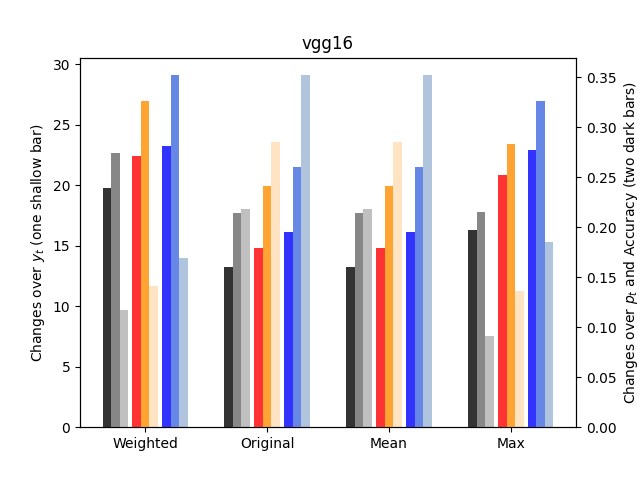
\includegraphics[width = 0.3\textwidth]{figures/grad_sign_perturbation/vgg16_eps003.png} &
    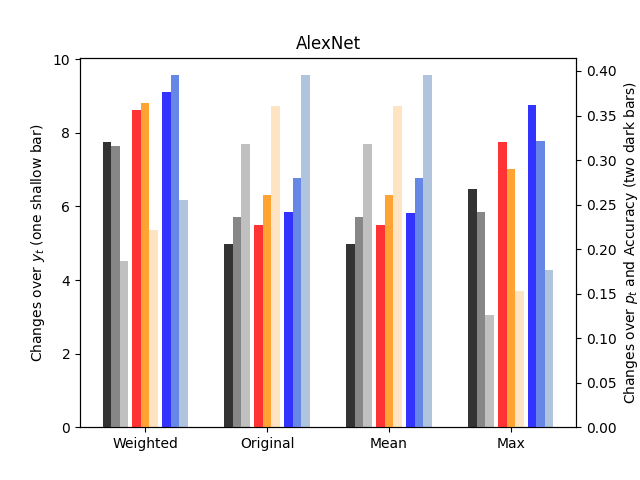
\includegraphics[width = 0.3\textwidth]{figures/grad_sign_perturbation/alexnet_eps003.png} &
    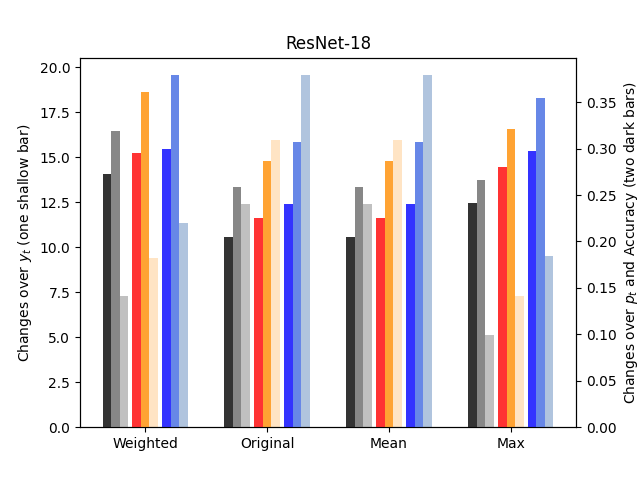
\includegraphics[width = 0.3\textwidth]{figures/grad_sign_perturbation/resnet18_eps003.png} \\

    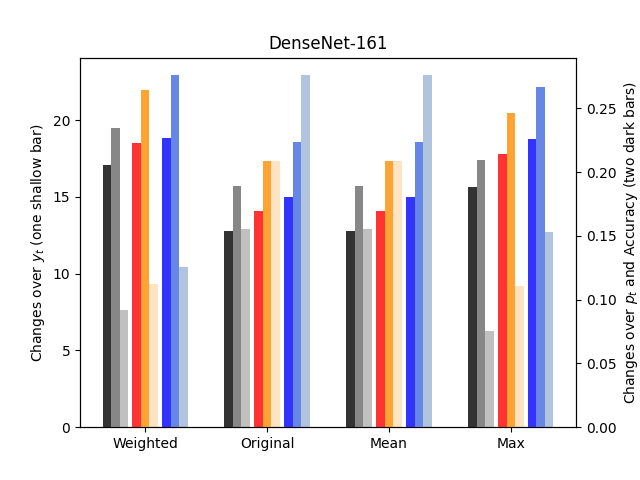
\includegraphics[width = 0.3\textwidth]{figures/grad_sign_perturbation/densenet161_eps003.png} &
    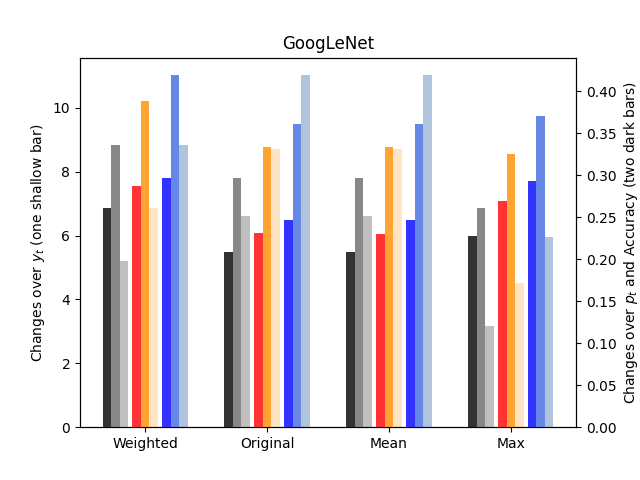
\includegraphics[width = 0.3\textwidth]{figures/grad_sign_perturbation/googlenet_eps003.png} &
    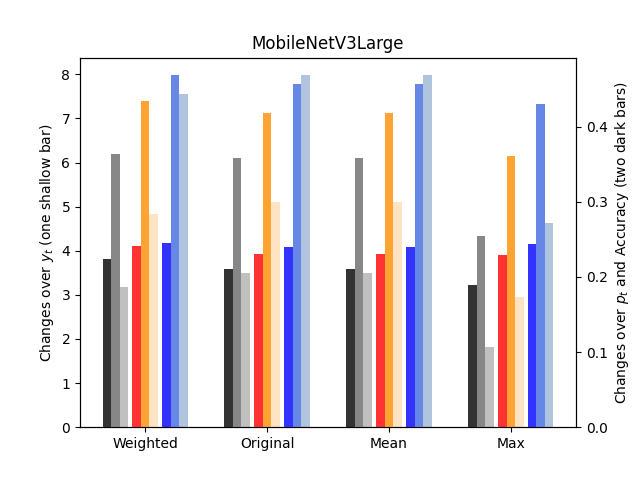
\includegraphics[width = 0.3\textwidth]{figures/grad_sign_perturbation/mobilenetv3large_eps003.png} \\

    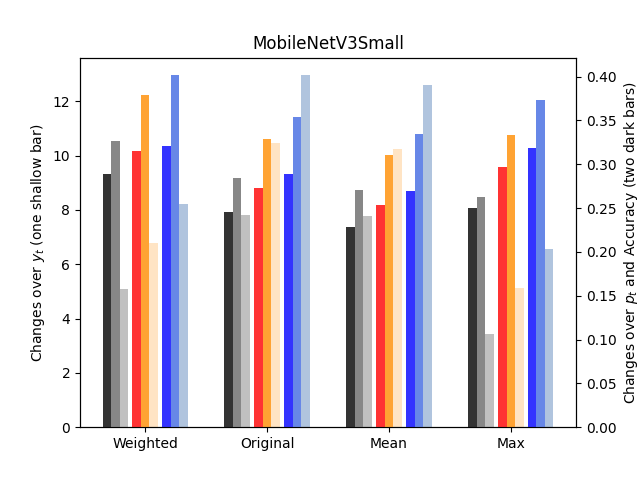
\includegraphics[width = 0.3\textwidth]{figures/grad_sign_perturbation/mobilenetv3small_eps003.png} &
    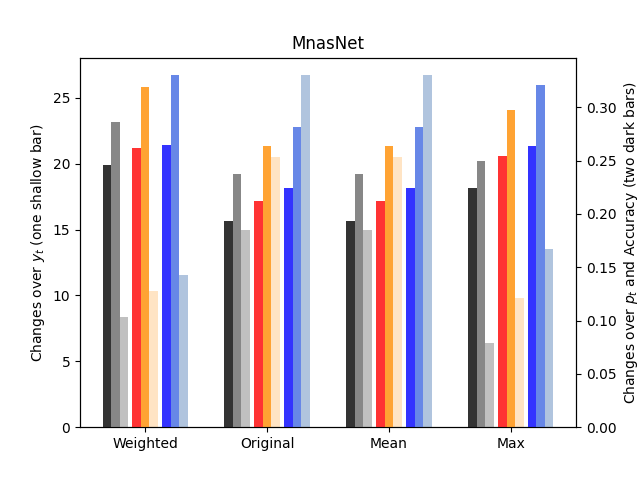
\includegraphics[width = 0.3\textwidth]{figures/grad_sign_perturbation/mnasnet_eps003.png} &
    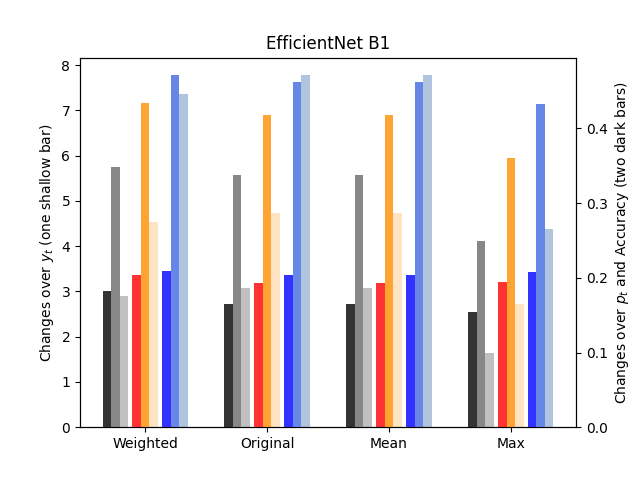
\includegraphics[width = 0.3\textwidth]{figures/grad_sign_perturbation/efficientnetB1_eps003.png} \\

\multicolumn{3}{c}{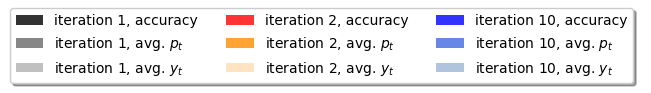
\includegraphics[width = 0.7\textwidth]{figures/grad_sign_perturbation/legend.png} }\\
\end{tabular}
\caption{Reproducing of Figure 3 in the original paper with $\epsilon=\num{3e-3}$. Changes in accuracy, $y_t$ and $p_t$ (t is the target classification class) when certain input features are perturbed. Perturbed features are selected based on four gradient explanations (original, mean, max and weighted), where original is directly with respect to the gradients of the logits.} \label{f:grad_sign_perturbation_eps_003}
\end{figure}